
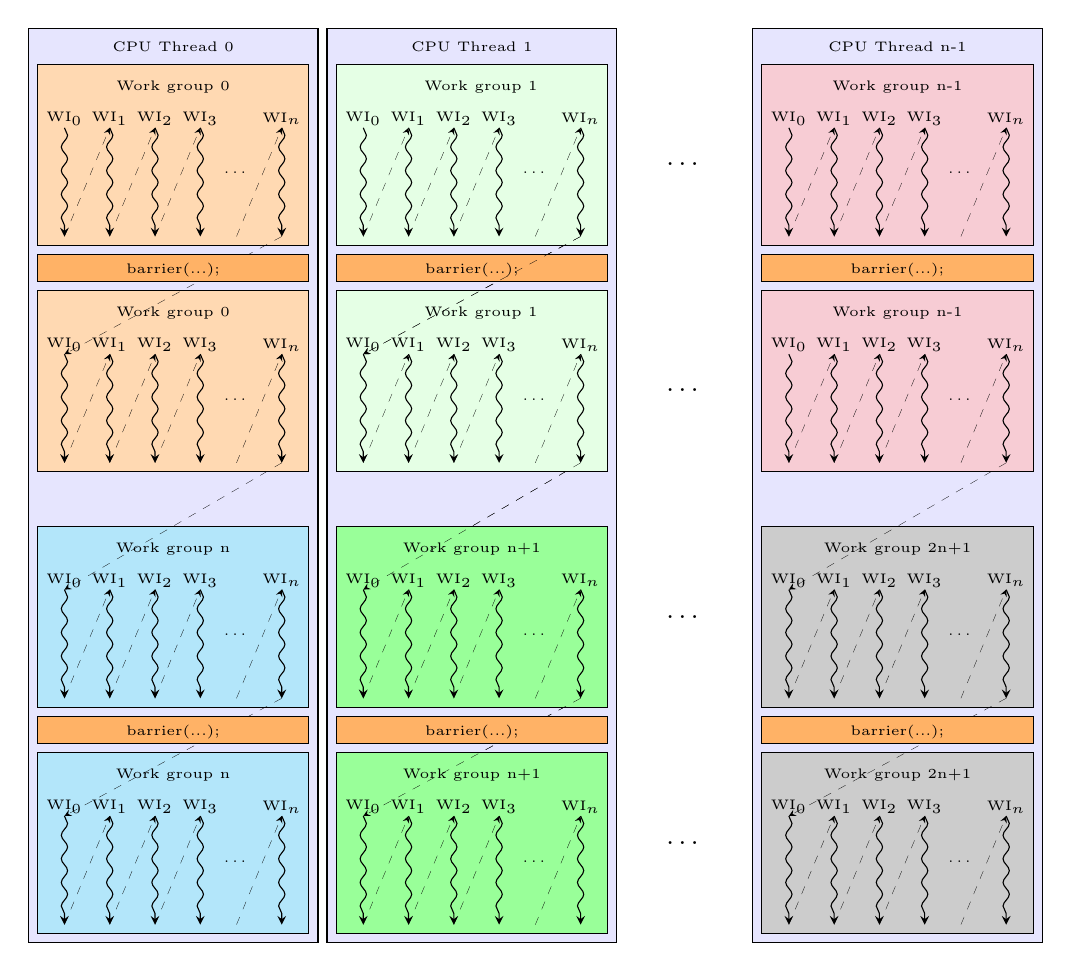
\begin{tikzpicture}[ scale=1.15,
  >=stealth,
  snaky/.style={->,decorate,decoration={name=snake,amplitude=.4mm,segment length=3mm,post length=0.5mm}},
  dashy/.style={->,dashed,ultra thin}
]
\usetikzlibrary{scopes}
\usetikzlibrary{decorations,snakes}

\foreach \x/\xtext in {0/0,3.3/1, 8/n-1}
{
  \draw[fill=purple!5!blue!10] (\x,10) rectangle ++(3.2,-10.1);
  \draw[font=\tiny] node at (\x+3.2/2, 9.8) {CPU Thread \xtext};
}

\def\wavylines#1#2{
\begin{scope}[xshift=#1,yshift=#2]


\draw node [font=\tiny] {WI$_0$};
\draw [snaky] (0,-0.1) -- ++(0,-1.2);

\foreach \x in {1,2,3}
{
  \draw node [font=\tiny] at (0.5*\x, 0) {WI$_\x$};
  \draw [dashy] ( \x*0.5 - 0.5, -1.3) -- ++(0.5,1.2);
  \draw [snaky] ( \x*0.5, -0.1) -- ++(0,-1.2);
}
\draw[font=\tiny] node at (1.9,-0.6) {\ldots};
\draw node at (2.4,0) [font=\tiny] {WI$_n$};
\draw [snaky] (2.4,-0.1) -- ++(0,-1.2);
\draw [dashy] (1.9,-1.3) -- ++(0.5,1.2); 

\end{scope}
} %wavylines

%CPU thread 0

% Work group 0
\draw[fill=orange!30] (0.1,9.6) rectangle ++(3,-2.0);
\draw[font=\tiny] node at (3.2/2, 9.35) {Work group 0};
\wavylines{0.4cm}{9.0cm};

\draw[fill=orange!30] (0.1,7.1) rectangle ++(3,-2.0);
\draw[font=\tiny] node at (3.2/2, 6.85) {Work group 0};
\wavylines{0.4cm}{6.5cm};

\draw[dashy] (2.8,7.7) -- (0.4,6.4);

\draw[fill=orange!60] (0.1,7.5) rectangle ++(3,-0.3);
\draw[font=\tiny] node at (1.6, 7.33) {barrier(...);};

% Work group 1
\draw[fill=cyan!30] (0.1,4.5) rectangle ++(3,-2.0);%CPU thread 1

% Work group 0
\draw[fill=green!10] (3.4,9.6) rectangle ++(3,-2.0);
\draw[font=\tiny] node at (3.4+3.2/2, 9.35) {Work group 1};
\wavylines{3.7cm}{9.0cm};

\draw[fill=green!10] (3.4,7.1) rectangle ++(3,-2.0);
\draw[font=\tiny] node at (3.4 + 3.2/2, 6.85) {Work group 1};
\wavylines{3.7cm}{6.5cm};

\draw[dashy] (3.3 + 2.8,7.7) -- (3.7,6.4);

\draw[fill=orange!60] (3.4,7.5) rectangle ++(3,-0.3);
\draw[font=\tiny] node at (3.3+1.6, 7.33) {barrier(...);};

% Work group 1
\draw[fill=green!40] (3.4,4.5) rectangle ++(3,-2.0);
\draw[font=\tiny] node at (3.3+3.2/2, 4.25) {Work group n+1};
\wavylines{3.7cm}{3.9cm};

\draw[dashy] (3.3+2.8,5.2) -- (3.3+0.4,3.8);

\draw[fill=green!40] (3.3+0.1,2.0) rectangle ++(3,-2.0);
\draw[font=\tiny] node at (3.3+3.2/2, 1.75) {Work group n+1};
\wavylines{3.7cm}{1.4cm};

\draw[dashy] (3.3+2.8,2.6) -- (3.3+0.4,1.3);

\draw[fill=orange!60] (3.3+0.1,2.4) rectangle ++(3,-0.3);
\draw[font=\tiny] node at (3.3+1.6, 2.23) {barrier(...);};
\draw[font=\tiny] node at (3.2/2, 4.25) {Work group n};
\wavylines{0.4cm}{3.9cm};

\draw[dashy] (2.8,5.2) -- (0.4,3.8);

\draw[fill=cyan!30] (0.1,2.0) rectangle ++(3,-2.0);
\draw[font=\tiny] node at (3.2/2, 1.75) {Work group n};
\wavylines{0.4cm}{1.4cm};

\draw[dashy] (2.8,2.6) -- (0.4,1.3);

\draw[fill=orange!60] (0.1,2.4) rectangle ++(3,-0.3);
\draw[font=\tiny] node at (1.6, 2.23) {barrier(...);};

%CPU thread 1

% Work group 0
\draw[fill=green!10] (3.4,9.6) rectangle ++(3,-2.0);
\draw[font=\tiny] node at (3.4+3.2/2, 9.35) {Work group 1};
\wavylines{3.7cm}{9.0cm};

\draw[fill=green!10] (3.4,7.1) rectangle ++(3,-2.0);
\draw[font=\tiny] node at (3.4 + 3.2/2, 6.85) {Work group 1};
\wavylines{3.7cm}{6.5cm};

\draw[dashy] (3.3 + 2.8,7.7) -- (3.7,6.4);

\draw[fill=orange!60] (3.4,7.5) rectangle ++(3,-0.3);
\draw[font=\tiny] node at (3.3+1.6, 7.33) {barrier(...);};

% Work group 1
\draw[fill=green!40] (3.4,4.5) rectangle ++(3,-2.0);
\draw[font=\tiny] node at (3.3+3.2/2, 4.25) {Work group n+1};
\wavylines{3.7cm}{3.9cm};

\draw[dashy] (3.3+2.8,5.2) -- (3.3+0.4,3.8);

\draw[fill=green!40] (3.3+0.1,2.0) rectangle ++(3,-2.0);
\draw[font=\tiny] node at (3.3+3.2/2, 1.75) {Work group n+1};
\wavylines{3.7cm}{1.4cm};

\draw[dashy] (3.3+2.8,2.6) -- (3.3+0.4,1.3);

\draw[fill=orange!60] (3.3+0.1,2.4) rectangle ++(3,-0.3);
\draw[font=\tiny] node at (3.3+1.6, 2.23) {barrier(...);};

\draw node at (7.25,8.5) {\ldots};
\draw node at (7.25,6) {\ldots};
\draw node at (7.25,3.5) {\ldots};
\draw node at (7.25,1.0) {\ldots};

%CPU thread n-1

% Work group 0
\draw[fill=blue!15!red!20] (8.1,9.6) rectangle ++(3,-2.0);
\draw[font=\tiny] node at (8+3.2/2, 9.35) {Work group n-1};
\wavylines{8.4cm}{9.0cm};

\draw[fill=blue!15!red!20] (8.1,7.1) rectangle ++(3,-2.0);
\draw[font=\tiny] node at (8 + 3.2/2, 6.85) {Work group n-1};
\wavylines{8.4cm}{6.5cm};

\draw[dashy] (3.3 + 2.8,7.7) -- (3.7,6.4);

\draw[fill=orange!60] (8.1,7.5) rectangle ++(3,-0.3);
\draw[font=\tiny] node at (8+1.6, 7.33) {barrier(...);};

% Work group 1
\draw[fill=gray!40] (8.1,4.5) rectangle ++(3,-2.0);
\draw[font=\tiny] node at (8+3.2/2, 4.25) {Work group 2n+1};
\wavylines{8.4cm}{3.9cm};

\draw[dashy] (8+2.8,5.2) -- (8+0.4,3.8);

\draw[fill=gray!40] (8+0.1,2.0) rectangle ++(3,-2.0);
\draw[font=\tiny] node at (8+3.2/2, 1.75) {Work group 2n+1};
\wavylines{8.4cm}{1.4cm};

\draw[dashy] (8+2.8,2.6) -- (8+0.4,1.3);

\draw[fill=orange!60] (8+0.1,2.4) rectangle ++(3,-0.3);
\draw[font=\tiny] node at (8+1.6, 2.23) {barrier(...);};

\end{tikzpicture}
